\let\negmedspace\undefined
\let\negthickspace\undefined
\documentclass[journal]{IEEEtran}
\usepackage[a5paper, margin=10mm, onecolumn]{geometry}
%\usepackage{lmodern} % Ensure lmodern is loaded for pdflatex
\usepackage{tfrupee} % Include tfrupee package

\setlength{\headheight}{1cm} % Set the height of the header box
\setlength{\headsep}{0mm}     % Set the distance between the header box and the top of the text

\usepackage{gvv-book}
\usepackage{gvv}
\usepackage{cite}
\usepackage{amsmath,amssymb,amsfonts,amsthm}
\usepackage{algorithmic}
\usepackage{graphicx}
\usepackage{textcomp}
\usepackage{xcolor}
\usepackage{txfonts}
\usepackage{listings}
\usepackage{enumitem}
\usepackage{mathtools}
\usepackage{gensymb}
\usepackage{comment}
\usepackage[breaklinks=true]{hyperref}
\usepackage{tkz-euclide} 
\usepackage{listings}
% \usepackage{gvv}                                        
\def\inputGnumericTable{}                                 
\usepackage[latin1]{inputenc}                                
\usepackage{color}                                            
\usepackage{array}                                            
\usepackage{longtable}                                       
\usepackage{calc}                                             
\usepackage{multirow}                                         
\usepackage{hhline}                                           
\usepackage{ifthen}                                           
\usepackage{lscape}
\begin{document}

\bibliographystyle{IEEEtran}
\vspace{3cm}

\title{CHAPTER - 7\\Circle}
\author{EE24BTECH11061 - Rohith Sai}
% \maketitle
% \newpage
% \bigskip
{\let\newpage\relax\maketitle}

\renewcommand{\thefigure}{\theenumi}
\renewcommand{\thetable}{\theenumi}
\setlength{\intextsep}{10pt} % Space between text and floats

\numberwithin{figure}{enumi}
\renewcommand{\thetable}{\theenumi}

\section{7.3 Miscellaneous}
\begin{enumerate}
\item [7.3.6] The equation of the circle circumscribing the triangle whose sides are the lines
$y = x + 2$, $3y = 4x$, $2y = 3x$ is\\
\textbf{Solution:}
The given lines are
\begin{align}
    \myvec{1 & -1} \vec{x} = -2\\
    \myvec{4 & -3} \vec{x} = 0\\
    \myvec{3 & -2} \vec{x} = 0
\end{align}
The points of intersection of the lines are given as $A, B, C$
\begin{align}
    \vec{a} = \myvec{1 & -1 & \mid & -2\\4 & -3 & \mid & 0}\\
    \implies \vec{a} = \myvec{6\\8}\\
    \vec{b} = \myvec{4 & -3 & \mid & 0\\3 & -2 & \mid & 0}\\
    \implies \vec{b} = \myvec{0\\0}\\
    \vec{c} = \myvec{3 & -2 & \mid & 0\\1 & -1 & \mid & -2}\\
    \implies \vec{c} = \myvec{4\\6}
\end{align}
\begin{table}[h!]
      \centering
      \begin{tabular}[12pt]{ |c| c|}
    \hline
    \textbf{Variable} & \textbf{Description}\\ 
    \hline
    $x\brak{0}$ & First term of the AP \\
    \hline 
    $d$ & Common difference of the AP\\
    \hline
    $y\brak{n}$ & Sum of $n+1$ terms of the AP\\
    \hline
    $x\brak{n}$ & General term\\
    \hline   
    \end{tabular}
      \caption{}
\end{table}\\
Now we need to find the equation of the circle passing these three vertices $A, B, C$
\begin{align}
    \myvec{2\vec{a} & 2\vec{b} & 2\vec{c}\\1 & 1 & 1}^\top \myvec{\vec{u}\\f} = -\myvec{\abs{\abs{\vec{a}}}^2\\\abs{\abs{\vec{b}}}^2\\\abs{\abs{\vec{c}}}^2}
\end{align}
Substituting the numerical values, we get
\begin{align}
    \myvec{12 & 16 & 1\\0 & 0 & 1\\8 & 12 & 1}\myvec{\vec{u}\\f} = \myvec{-100\\0\\-52}\\
    \implies \vec{u} = \myvec{-23\\11}\\f = 0
\end{align}
For the given values, the circle is represented as
\begin{figure}[h!]
    \centering
    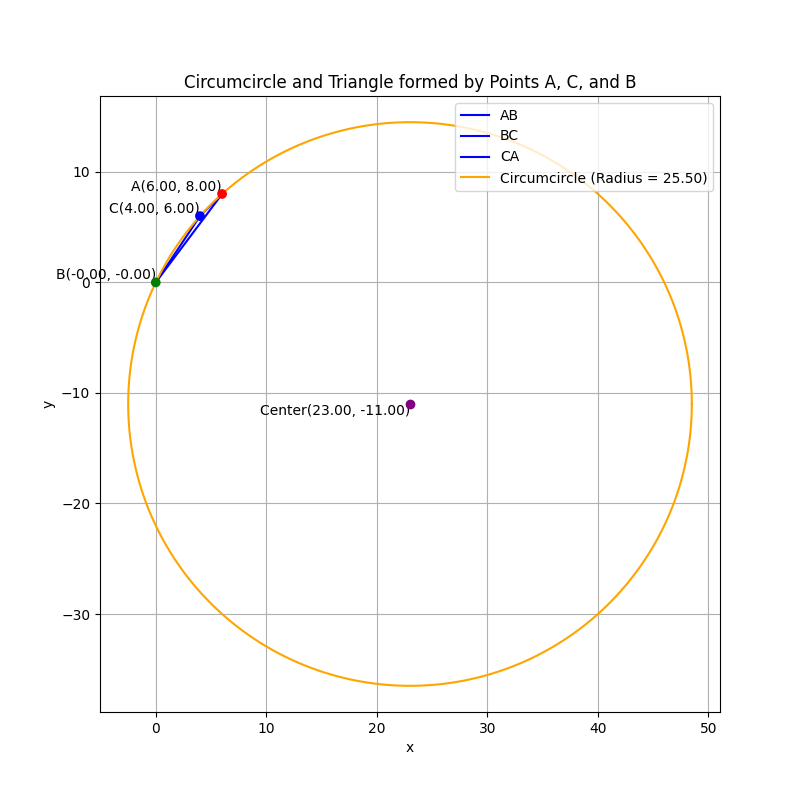
\includegraphics[width=10cm]{figs/figure.png}
    \caption{}
    \label{fig:enter-label}
\end{figure}
\end{enumerate}
\end{document}